\section{Capture Mismatch, Temporal Evidence, and Delivery}
\label{sec:mismatch}
The mismatch experiment asks whether retained observations remain useful
when the downstream receiver differs from the capture trigger. We compare
first-difference, standardized-level, and PCA-guided capture, plus an explicitly
disabled trigger as a stress control. Level capture uses the existing six-standard-
deviation threshold; PCA capture reaches the same trigger boundary at its frozen
training score quantile. Each condition drives threshold-only capture, the existing
adaptive recorder, and a coverage-based background control. Uniform and ten-seed
reservoir/random-phase controls complete 132 arms across the four caps.
Original pilot and seeded streams are hash-verified and reused.

The receiver bank contains standardized level and PCA residuals at ranks one
through five. All additional calibration uses eligible training observations only;
the original level and rank-three parameters remain exact. PCA ranks are correlated
sensitivity checks, not independent detector families or fault examples. All
source-eligible events stay in the denominator, and each receiver separately reports
full-archive recoverability and losses caused by retention.

\paragraph{Coverage control.}
Within each reserved background time stratum, a bounded candidate replaces its
background observation when a new observation is further from the already retained
background observations in frozen standardized units. Records requested by trigger
or context capture are protected. The candidate uses the same reserved quota and
wire schema. This is an experimental diversity control, not a claim of a novel
streaming selection algorithm or an optimal allocation.

\begin{table}[htbp]
\centering
\scriptsize
% Generated from completed receiver mismatch benchmark.
\begin{tabular}{llrrrr}
\toprule
Capture & Policy & MiB & PCA events & Blind kept/available & Pre-context (\%) \\
\midrule
Difference & Threshold & 0.81 & 10/11 & 0/1 & 0.0 \\
Difference & Adaptive & 6.30 & 11/11 & 1/1 & 64.3 \\
Difference & Coverage & 6.30 & 11/11 & 1/1 & 66.3 \\
Level & Threshold & 1.38 & 10/11 & 0/1 & 0.0 \\
Level & Adaptive & 6.67 & 11/11 & 1/1 & 65.1 \\
Level & Coverage & 6.67 & 11/11 & 1/1 & 67.1 \\
PCA & Threshold & 1.58 & 11/11 & 0/0 & 0.0 \\
PCA & Adaptive & 8.86 & 11/11 & 0/0 & 65.1 \\
PCA & Coverage & 8.75 & 11/11 & 0/0 & 66.3 \\
Disabled & Threshold & 0.80 & 0/11 & 0/11 & 0.0 \\
Disabled & Adaptive & 6.22 & 4/11 & 4/11 & 1.8 \\
Disabled & Coverage & 6.22 & 6/11 & 6/11 & 2.9 \\
\bottomrule
\end{tabular}

\caption{Capture mismatch at the 1,024-byte hourly cap. ``Blind'' means no
capture threshold crossing within the event; nearby triggers can still preserve
context. The conditional denominator includes only full-archive PCA-recoverable
events. All 11 source-eligible events remain in the overall event denominator.}
\label{tab:mismatch}
\end{table}

With first-difference capture, both adaptive and coverage recorders retain
rank-three PCA evidence for 11/11 events at approximately 6.30 MiB. Coverage
increases pre-context from 64.3\% to 66.3\% but reduces post-context from 40.2\%
to 36.9\%. At ranks four and five, the original adaptive recorder retains 10/11
events and the coverage control retains 11/11. With the trigger disabled, they
retain rank-three evidence for 4/11 and 6/11 events respectively at 6.22 MiB.
These differences concern the same small validation archive, not evidence of
robustness to an arbitrary future model.

\paragraph{A distinct temporal receiver.}
We fit a ridge AR(1) model on 8,712,785 eligible consecutive training pairs,
with regularization 0.001, a 150-second gap reset, and a training score quantile
of 0.999. Scores use standardized forecast residuals. Both original endpoints
must survive for a transition to supply evidence: retained samples separated by
discarded observations are never silently stitched together. The full archive
contains temporal evidence for all 11 eligible events. Seven declared policies
at four caps give 28 temporal evaluations.

At 1,024 bytes, the existing adaptive recorder retains temporal evidence for
10/11 events, compared with 2/11 for uniform and 1/11 for threshold-only capture.
Disabling the trigger leaves singleton adaptive background capture with 0/11
temporal events despite its 4/11 pointwise PCA result. This exposes a limitation
of equating isolated retained values with evidence for a temporal receiver.

After observing this validation failure, we implement an adjacent-pair background
control and run eight exploratory arms. It reserves the same fraction of raw
capacity for pairs within time strata, rejects partners beyond the gap limit,
and never pairs across epochs. Odd unused quota slots remain unfilled. With
first-difference triggers, it retains 10/11 temporal events at the 1,024-byte cap,
matching the original recorder. With the trigger disabled, it retains 2/11 temporal
and 4/11 PCA events at 6.22 MiB. This partially addresses the measured failure,
not the general problem of preserving every unfamiliar fault. Its design is
informed by validation outcomes and requires independent confirmation.

\begin{table}[htbp]
\centering
\small
% Generated temporal receiver and adjacent-pair comparison.
\begin{tabular}{lrrrr}
\toprule
Capture / policy & MiB & PCA events & AR(1) events & Retained pairs \\
\midrule
Uniform & 25.04 & 5/11 & 2/11 & 2957 \\
Diff. / threshold & 0.81 & 10/11 & 1/11 & 11 \\
Diff. / adaptive & 6.30 & 11/11 & 10/11 & 1057 \\
Diff. / coverage & 6.30 & 11/11 & 10/11 & 4886 \\
Level / adaptive & 6.67 & 11/11 & 10/11 & 7281 \\
Pca / adaptive & 8.86 & 11/11 & 10/11 & 69167 \\
Disabled / adaptive & 6.22 & 4/11 & 0/11 & 0 \\
Diff. / burst & 6.30 & 11/11 & 10/11 & 79668 \\
Disabled / burst & 6.22 & 4/11 & 2/11 & 78877 \\
\bottomrule
\end{tabular}

\caption{Temporal receiver comparison at 1,024 bytes per hour. Retained pairs
require consecutive original observations within the gap limit. Burst rows are
exploratory additions after inspecting the temporal validation result.}
\label{tab:temporal}
\end{table}

\paragraph{Delivered rather than merely captured evidence.}
A store-and-forward simulator adds finite payload buffers, drop-oldest/drop-newest
rules, discrete contacts, partial transfer progress, framing costs, and completed-
packet loss. Arrivals at epoch end enter before service at the same timestamp.
Undelivered packets at evaluation end provide no evidence. Packet and payload
conservation are checked, and only completely delivered packets reach evaluation.
The model abstracts physical frame timing and does not implement retransmission.

Illustrative contacts occur every six hours. Ample/lossy conditions allow 32,768
wire bytes per contact and a 16,384-byte payload buffer; congestion allows 2,048
and 4,096 bytes. Every 128 payload bytes incur 16 framing bytes. The lossy case
uses probability 0.1 and one declared seed. At 1,024 bytes, congestion reduces
uniform PCA evidence from 5/11 to 4/11 while adaptive and coverage retain 11/11;
the lossy realization reduces both latter policies to 10/11. These schedules
are not validated mission requirements and one loss seed is not an uncertainty
analysis. Congestion differences combine selection with differing actual
expenditure; they do not isolate transport robustness at matched byte cost. Buffer limits exclude Python object metadata.

\begin{table}[htbp]
\centering
\small
% Generated finite-buffer delivery comparison.
\begin{tabular}{llrrr}
\toprule
Policy & Link & Wire MiB & Delivered packets & PCA events \\
\midrule
Uniform & Ample & 28.24 & 26304/26304 & 5/11 \\
Uniform & Congested & 8.56 & 4498/26304 & 4/11 \\
Uniform & Lossy & 28.24 & 23638/26304 & 5/11 \\
Adaptive & Ample & 7.11 & 26304/26304 & 11/11 \\
Adaptive & Congested & 7.04 & 26182/26304 & 11/11 \\
Adaptive & Lossy & 7.11 & 23638/26304 & 10/11 \\
Coverage & Ample & 7.11 & 26304/26304 & 11/11 \\
Coverage & Congested & 7.04 & 26182/26304 & 11/11 \\
Coverage & Lossy & 7.11 & 23638/26304 & 10/11 \\
\bottomrule
\end{tabular}

\caption{Encoded evidence after illustrative finite-buffer delivery, at the
1,024-byte hourly recording cap. Wire cost includes framing and unsuccessful
or partial transmissions; it differs from encoded capture expenditure.}
\label{tab:delivery}
\end{table}

\begin{figure}[htbp]
\centering
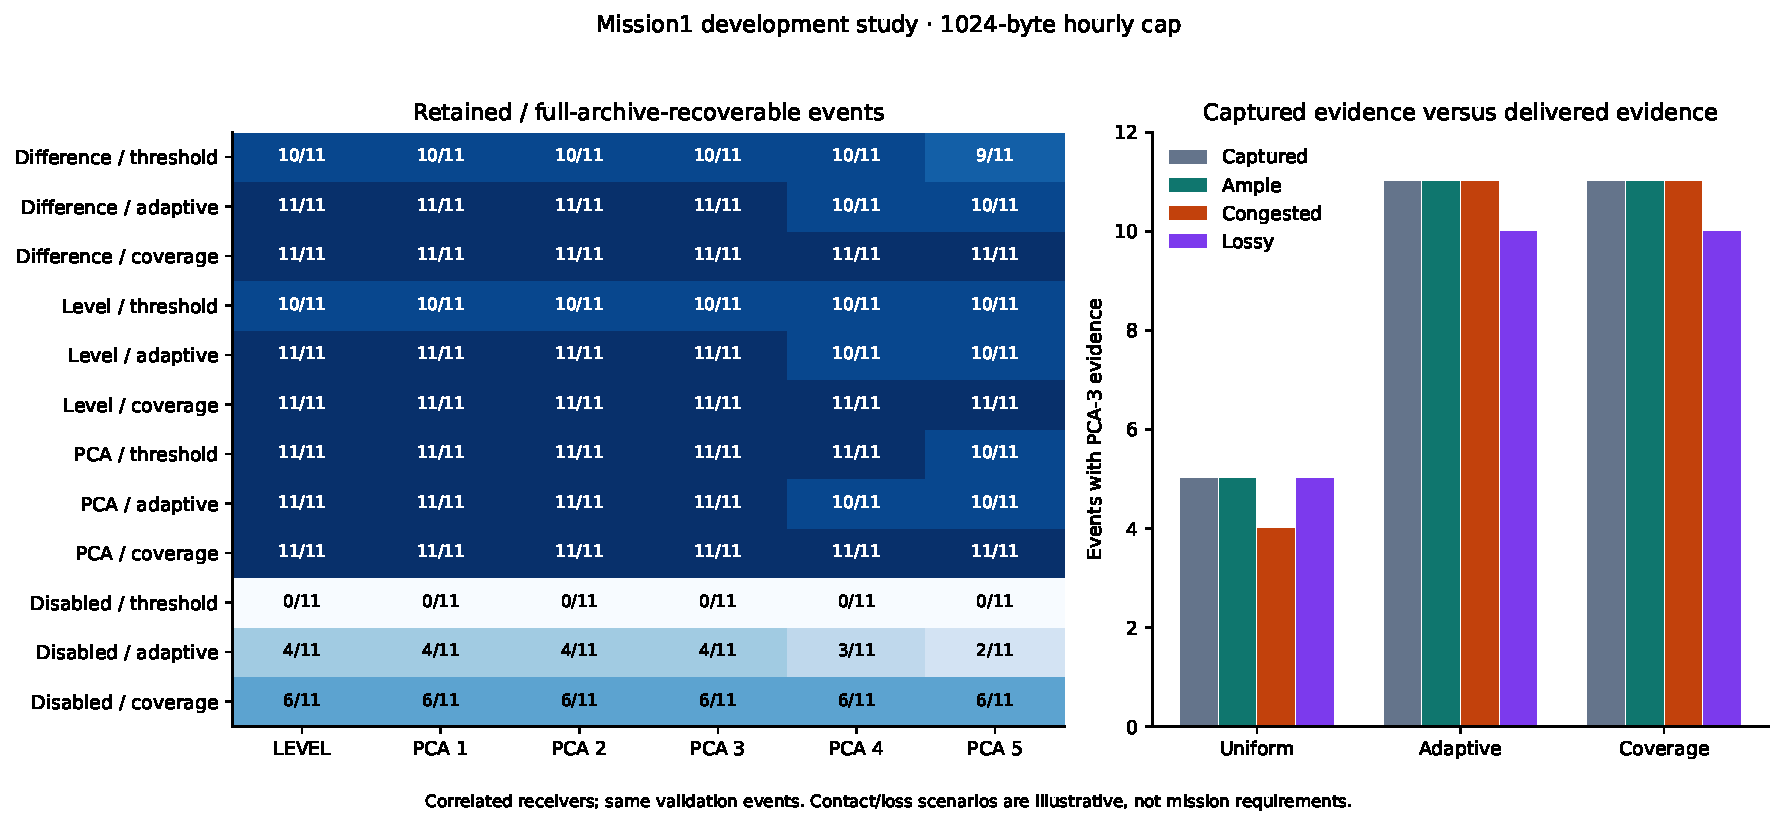
\includegraphics[width=\linewidth]{generated/receiver_mismatch.pdf}
\caption{Receiver sensitivity and captured/delivered evidence on the same
Mission1 validation events. Matrix denominators are receiver-specific full-archive
recoverability. Neither the correlated receivers nor the link scenarios establish
independent-mission generalization.}
\label{fig:mismatch}
\end{figure}

\paragraph{Reproducibility and resource scope.}
The independent-mission benchmark now locks input, canonical settings, code and
requirements hashes, and Python/NumPy versions. It reports 148 default capture
arms including adjacent-pair controls, followed by 36 selected temporal evaluations.
Only synthetic external bundles have been exercised; an independent mission result
remains pending. A separate 20,000-observation host profile measures replay timing
and Python-traced allocations in different passes. On this local run, adaptive
replay processes approximately 396,000 observations per second and coverage
approximately 104,000, including synthetic sample construction, encoding, and
hashing. These are single-run host measurements under a local development
workload, not embedded latency, total RAM, or flight suitability evidence.
